\section{试运行与停止}
\label{sec:budget-stopping}

前面的分配与选择都用到了事先不知道的量：单样本方差、成本、包络常数、$\tau_{f}$、建议分布的参数。它们只能由试运行估计。试运行的结果一旦用来做决定，后面的计算就依赖于这些随机的决定，原先对固定方法证明的结论是否还成立，需要重新检查。同样的问题出现在“何时停止”上：按事先固定的样本数停止，与看着结果决定何时停止，是两种不同的随机程序。

\paragraph{试运行与正式计算分开}
试运行的作用是估计成本、波动以及方法的参数，例如图~\ref{fig:budget-pilot-size}中的$\hat{\lambda}$、式~\eqref{eq:budget-neyman-cost}中的$\sigma_k$、图~\ref{fig:budget-sampler-costs}中的步长。正式计算用新的独立随机数。这样，给定试运行结果时，正式计算就是一个参数固定的普通方法，第~\ref{chap:monte-carlo-integration-error}章和第~\ref{chap:variance-reduction}章对固定方法证明的无偏性、方差公式和渐近区间都可以在条件意义下直接使用。

试运行的样本可不可以并入最终的平均？若试运行只是从固定的分布抽样且不参与任何选择，并入没有问题。若试运行被用来在几个方法中挑选，问题就来了：设对两个同样无偏的方法各做一次试运行，选估计方差较小的一个，再报告它在试运行中的估计。被选中的往往是试运行时“碰巧波动较小”的那一个，而对偏斜的被积函数，波动偏小常常伴随着均值偏小（漏掉了大的贡献），于是报告的数系统地偏低。最稳妥的做法是只把试运行用于决定，最终估计只用正式计算的样本；试运行所占的预算按式~\eqref{eq:budget-pilot-opt}本来就只是一小部分。

\paragraph{固定转移核与持续调参}
MCMC的步长、提议协方差等参数通常靠试运行调整。调整的依据应当是第~\ref{sec:budget-costs}节的$c_{\mathrm{it}}\tau_{f}$，而不只是接受率：图~\ref{fig:budget-sampler-costs}中接受率最高的$s=1$恰恰最贵。试运行结束后把参数固定，正式计算的链就是一条时间齐次的Markov链，转移核保持目标不变；但链是否从初值的影响中走出来、是否走遍目标、相关误差多大，仍要按第~\ref{chap:monte-carlo-integration-error}章逐项核对，参数选得好并不能免除这些检查。

一个诱人的做法是不停止调参：在正式计算中继续根据已走过的轨迹修改转移核。每个可能用到的核都以$\pi$为不变分布，看起来整体也应当正确。下面的例子说明这个推理不成立。状态空间为$\{1,2\}$，目标$\pi=(\tfrac12,\tfrac12)$。核$K_{A}$是恒等转移（停在原处），核$K_{B}$以概率$\tfrac12$去往每个状态，二者都保持$\pi$不变：
\[
  \pi K_{A}=\pi,\qquad\pi K_{B}=\bigl(\tfrac12,\tfrac12\bigr)=\pi .
\]
调整规则是：当前在状态$1$时用$K_{A}$，在状态$2$时用$K_{B}$。图~\ref{fig:budget-adaptive-trap}画出两个核及其组合。

\begin{BookInlineFigure}
  \centering
  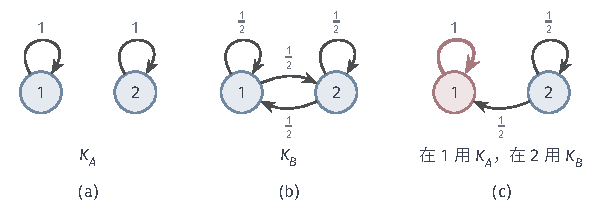
\includegraphics[width=101mm]{figures/07-probability/08-sampling-and-integration/tikz/budget-adaptive-trap/figure.pdf}
  \caption{每个核都保持目标不变，按轨迹选核却可能破坏它。状态空间$\{1,2\}$，目标$\pi=(\tfrac12,\tfrac12)$。(a)~$K_{A}$为恒等转移。(b)~$K_{B}$的每个转移概率都是$\tfrac12$。(c)~在状态$1$用$K_{A}$、在状态$2$用$K_{B}$的组合：状态$1$（红）成为吸收态。}
  \label{fig:budget-adaptive-trap}
\end{BookInlineFigure}

组合后的过程从状态$1$出发永远停在$1$，从状态$2$出发每步以$\tfrac12$的概率跳到$1$并从此停住。从$\pi$启动，$\mathbb{P}(X^{(0)}=2)=\tfrac12$，此后每步留在$2$的概率为$\tfrac12$，所以
\[
  \mathbb{P}\bigl(X^{(t)}=2\bigr)=\frac12\Bigl(\frac12\Bigr)^{t},\qquad\mathbb{P}\bigl(X^{(t)}=1\bigr)=1-2^{-(t+1)}\to1 .
\]
过程收敛到点质量$\delta_{1}$，而不是$\pi$。问题在于“用哪个核”依赖当前状态，组合起来的是另一个转移核，它不再保持$\pi$不变。不变性是对固定的核说的，不能由“每次所用的核都保持$\pi$”推出整体保持$\pi$。

持续调参并非不可行，但需要额外的理论。大致说，要求调整的幅度随时间趋于零，并且所用的核对目标的收敛速度有一致的控制，才能证明过程的边缘分布趋于$\pi$、平均满足大数律。这些条件涉及一般Markov链的遍历理论，证明较长，相关的收敛工具可参考\BookChapterRef{chap:discrete-time-stochastic-processes}{卷九第3章“离散时间随机过程”}。本卷采用更简单的做法：试运行中调参，正式计算中固定。

\paragraph{经验稳定的局限}
试运行和停止判断都要看结果是否“稳定”，但有限记录上的稳定不能证明正确。下面三种现象都会让运行均值在错误的值附近显得平稳。

第一种是稀有的大贡献。若对积分起主要作用的区域概率很小，有限的试运行可能一个样本也没有落进去，估计的方差为零，一切看起来都很精确。图~\ref{fig:budget-pilot-size}的例子之所以平稳，是因为$q_{0}=\operatorname{Exp}(1/2)$落入尾部的概率是$\mathrm{e}^{-2}\approx0.135$；若试运行直接从$\operatorname{Exp}(1)$抽样，这个概率只有$0.018$，$n_{0}=20$时有约$69\%$的试运行完全看不到尾部。

第二种是权重集中。仍算$I=\mathbb{P}(X>4)$，但用尾部比目标还轻的建议分布$q=\operatorname{Exp}(2.2)$。权重$w(y)=\mathrm{e}^{-y}/(2.2\,\mathrm{e}^{-2.2y})$在尾部指数增长，加权变量在$q$下的二阶矩为
\[
  \int_{4}^{\infty}\frac{\mathrm{e}^{-2y}}{2.2\,\mathrm{e}^{-2.2y}}\,\mathrm{d}y=\frac{1}{2.2}\int_{4}^{\infty}\mathrm{e}^{0.2y}\,\mathrm{d}y=\infty,
\]
估计无偏而方差无穷。图~\ref{fig:budget-weight-instability}画出三次独立运行：每次在前几千个样本内都没有命中尾部，估计为零；命中后估计跳起，之后每隔一段又被一个更大的权重抬升。$10^{6}$个样本后三次的估计约为$0.0149$、$0.0164$、$0.0163$，都低于$I\approx0.0183$。右图是最大的一项在累计和中的占比：它长时间接近$1$，说明整个估计由一两个样本决定。

\begin{BookInlineFigure}
  \centering
  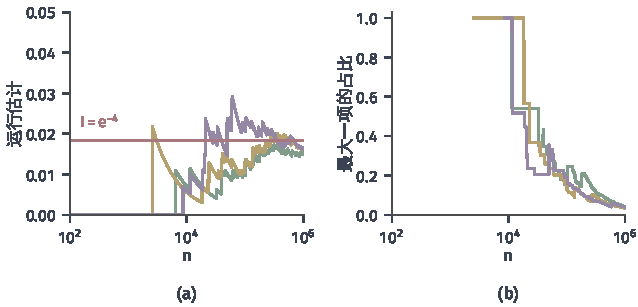
\includegraphics[width=108mm]{figures/07-probability/08-sampling-and-integration/matplotlib/budget-weight-instability/figure.pdf}
  \caption{建议分布尾部过轻时的重要性采样：目标$I=\mathbb{P}(X>4)$，$X\sim\operatorname{Exp}(1)$，从$\operatorname{Exp}(2.2)$抽样，加权变量方差无穷。三种颜色是三次独立运行（种子$11$、$12$、$13$）。(a)~运行估计，红线为真值。(b)~累计和中最大一项所占的比例。}
  \label{fig:budget-weight-instability}
\end{BookInlineFigure}

第三种是链之间的分歧。图~\ref{fig:budget-multistart}中每条链的运行均值都在某个值附近平稳下来，只有并排比较多条从不同初值出发的链，才看得出它们停在不同的地方。

这三种现象对应三种检查：对被积函数与建议分布的尾部做解析的矩估计，监视最大权重的占比，比较多条独立启动的链。它们能发现问题，但都不能证明没有问题：若所有链都错过了同一个峰，或所有试运行都没有触及同一个稀有区域，检查也全部通过。经验检查只能补充理论条件，不能代替它。

\paragraph{固定样本数与数据依赖的停止}
最常见的停止方式是看着误差估计做决定：每增加一些样本就计算一次$z\,s_n/\sqrt{n}$，一旦它小于容差$\varepsilon$就停止，报告$\bar{X}_n\pm z\,s_n/\sqrt{n}$。称这类规则为\term{序贯停止规则}（sequential stopping rule），停止时的样本数$N_{\varepsilon}$是随机的，依赖于样本本身。固定样本数的中心极限定理说的是$n$不随数据变化的情形，不能直接搬到$N_{\varepsilon}$上。

机制在偏斜分布上最清楚。设$f(U)=U^{-1/3}$，即$X$服从$[1,\infty)$上指数为$3$的Pareto分布，$I=1.5$，$\sigma^{2}=0.75$，右尾较重。一段样本恰好没有出现大值时，$s_n$偏小，均值也偏小；停止规则偏偏在这种时候触发，于是停下来时的估计系统地偏低，区间又偏窄。取$z=1.96$、最少$10$个样本、每增加一个样本检查一次，$20000$次模拟（种子$5$）的结果如图~\ref{fig:budget-sequential-coverage}。$\varepsilon=0.1$时，用真实$\sigma^{2}$定出的固定样本数$n=\lceil1.96^{2}\times0.75/0.01\rceil=289$，区间覆盖率约$0.925$；序贯规则平均只用了约$174$个样本就停止，覆盖率只有约$0.77$。

\begin{BookInlineFigure}
  \centering
  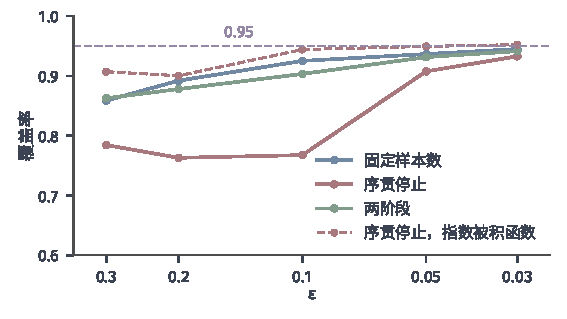
\includegraphics[width=96mm]{figures/07-probability/08-sampling-and-integration/matplotlib/budget-sequential-coverage/figure.pdf}
  \caption{名义$95\%$区间在三种停止方式下的实际覆盖率，横轴为目标半宽$\varepsilon$（向右减小）。实线为偏斜的被积函数$U^{-1/3}$（$I=1.5$，$\sigma^{2}=0.75$）：蓝线用真实方差定出固定样本数，红线在半宽首次小于$\varepsilon$时停止（最少$10$个样本），绿线先用$30$个独立试运行样本估计方差再定样本数。红色虚线为序贯停止用于$\mathrm{e}^{U}$的情形。每点$20000$次模拟（种子$5$）。}
  \label{fig:budget-sequential-coverage}
\end{BookInlineFigure}

$\varepsilon$变小时三条实线都向$0.95$靠拢：$\varepsilon=0.03$时固定样本数、两阶段与序贯规则的覆盖率分别约为$0.945$、$0.941$、$0.933$。对较对称的$\mathrm{e}^{U}$，序贯规则在$\varepsilon=0.1$时已有约$0.944$。这与一个渐近结论相符：若$0<\sigma^{2}<\infty$，并且停止规则要求的最少样本数随$\varepsilon\to0$趋于无穷（或在判据中加入防止过早停止的修正项），则$\varepsilon\to0$时覆盖率趋于名义值。它的证明需要随机样本数下的中心极限定理，篇幅较长，这里只说明其含义：数据依赖的停止只在误差要求足够严、停止时样本足够多时才近似可靠，对给定的有限$\varepsilon$没有保证。

既想依据数据定样本数、又要保留固定样本数的保证，可以把决定和估计分开，称为\term{两阶段方法}（two-stage procedure）：先用独立的试运行估计方差，据此定出正式样本数，再用新样本计算。

\begin{lemma}
\label{lem:budget-two-stage}
设试运行样本$\bm{Y}$与正式样本$X_1,X_2,\dots$相互独立，$X_i$独立同分布，$\mathbb{E}[X_i]=I$，$\operatorname{Var}(X_i)=\sigma^{2}<\infty$。正式样本数$N$是$\bm{Y}$的函数，取正整数值。令$\hat{I}=N^{-1}\sum_{i=1}^{N}X_i$，则
\begin{equation}
  \mathbb{E}\bigl[\hat{I}\mid\bm{Y}\bigr]=I,\qquad\operatorname{Var}\bigl(\hat{I}\mid\bm{Y}\bigr)=\frac{\sigma^{2}}{N},\qquad\operatorname{Var}(\hat{I})=\sigma^{2}\,\mathbb{E}\Bigl[\frac1N\Bigr].
  \label{eq:budget-two-stage}
\end{equation}
\end{lemma}

\begin{proof}
给定$\bm{Y}=\bm{y}$时$N=n(\bm{y})$是确定的正整数。由独立性，在这一条件下$X_1,X_2,\dots$的联合分布不变，仍独立同分布、均值$I$、方差$\sigma^{2}$。于是$n(\bm{y})$个样本的平均的条件期望为$I$，条件方差为$\sigma^{2}/n(\bm{y})$，这就是前两个等式。

由全期望公式，
\[
  \mathbb{E}[\hat{I}]=\mathbb{E}\bigl[\mathbb{E}[\hat{I}\mid\bm{Y}]\bigr]=I .
\]
由全方差公式，
\[
  \operatorname{Var}(\hat{I})=\mathbb{E}\bigl[\operatorname{Var}(\hat{I}\mid\bm{Y})\bigr]+\operatorname{Var}\bigl(\mathbb{E}[\hat{I}\mid\bm{Y}]\bigr)=\mathbb{E}\Bigl[\frac{\sigma^{2}}{N}\Bigr]+\operatorname{Var}(I)=\sigma^{2}\,\mathbb{E}\Bigl[\frac1N\Bigr],
\]
因为常数$I$的方差为零。
\end{proof}

引理的要点是$N$只依赖试运行。条件在试运行上，正式计算就是固定样本数的计算，固定样本数的渐近区间在条件意义下适用；$N$越大，条件覆盖率越接近名义值。图~\ref{fig:budget-sequential-coverage}的绿线用$30$个试运行样本的标准差$s_{0}$定出
\[
  N=\max\bigl\{30,\ \lceil z^{2}s_{0}^{2}/\varepsilon^{2}\rceil\bigr\},
\]
其覆盖率略低于用真实方差的蓝线（$\varepsilon=0.1$时约$0.903$对$0.925$），而明显高于序贯规则。差距来自试运行：$s_{0}$偏小时$N$偏小，最终区间可能比$\varepsilon$宽，也就是精度没有达标；但估计本身在条件意义下仍然无偏，不再出现序贯规则那种系统偏低。若$\bm{Y}$与正式样本不独立，例如把试运行样本并入最终平均，引理的条件就不满足。

用积分$\mathrm{e}-1$走一遍两阶段方法，取$\varepsilon=0.01$、$z=1.96$，随机数种子固定为$2026$。$30$个试运行样本的标准差为$s_{0}\approx0.426$，比真实的$\sigma\approx0.492$偏小，于是
\[
  N=\Bigl\lceil\frac{1.96^{2}\times0.426^{2}}{10^{-4}}\Bigr\rceil=6984,
\]
少于用真实方差算出的约$9300$。用新的$6984$个样本得到均值约$1.7290$，标准差约$0.493$，区间半宽为
\[
  1.96\times\frac{0.493}{\sqrt{6984}}\approx0.0116 .
\]
半宽超过了要求的$0.01$，这是试运行低估方差的后果；但这个区间如实反映了正式样本的波动，其下端约为$1.7174$，覆盖了$\mathrm{e}-1\approx1.7183$。若精度必须达标，可以把这次结果当作新的试运行，再定一次样本数，并仍用新样本计算。

最后，“预算用完就停”是固定预算的停止，样本数不依赖于样本的取值，固定样本数的结论适用。若每个样本的成本本身随机（例如拒绝采样的候选数），按预算停止时的样本数也随机，但它只依赖成本，不依赖被积函数的取值；拒绝采样中接受与否与被接受样本的取值独立，这种停止不会造成上面那种偏差。
